\documentclass{article}

\usepackage{fullpage}
\usepackage{pgf}
\usepackage{tikz}
\usepackage{hyperref}
\usepackage{fancyvrb}


\begin{document}
\title{Using Side-Effect Attributes}
\author{Anatole Le (\htmladdnormallink{ale44@sable.mcgill.ca}
        {mailto:ale44@sable.mcgill.ca})}
\date{\today}
\maketitle

This note explains how to use Soot annotation options to add
side-effect attributes in class files and
how these attributes can be used in JIT or ahead-of-time compilers.

\section{Side-Effects}

Side-effect analysis provides an approximation of the set of memory 
locations that each instruction may read or write. This analysis can 
optimize code by eliminating redundant loads and stores. It has been 
observed in the past for languages such as Modula-3, C or Java that 
the use of side-effect information 
in compilers does have a significant impact on performance.

Soot can perform static analyses for computing side-effect information
with different levels of precision. The simplest, 
least precise side-effect analysis computed in Soot 
uses Class Hierarchy Analysis (CHA) for an approximation of the call 
graph and method summaries of fields read and written. More precise 
(though more expensive) side-effect analyses 
make use of call graph and points-to information computed
by Spark. The results of these analyses can then be encoded in
class files as attributes, and ahead-of-time or JIT compilers can 
use it to improve optimizations such as common sub-expression
elimination, load elimination,
dead store removal and loop-invariant code motion. 

Soot also supports user-defined attributes.
The process of adding new analyses and attributes is documented in
``Adding attributes to class files via Soot''.

\section{Annotation Options for Side-Effects in Soot}

\subsection{Options}

Soot has a command-line option {\tt-annot-side-effect} 
to annotate class files with side-effect attributes. Since
a side-effect analysis requires a call-graph, options
whole-program mode ({\tt -w}) and application mode ({\tt -app}) must
also be specified. These three options are
required to perform Soot's simplest side-effect analysis, which we
call {\tt CHA}.

More precise side-effect analyses that make use of points-to
analysis can be computed using
various Spark options such as {\tt on-fly-cg} and {\tt field-based}.
When {\tt on-fly-cg} is true, the call graph is computed 
on the fly (otf) as the points-to analysis is performed. When it is false, it is
computed ahead-of-time (aot) using CHA. The {\tt field-based} option
specifies whether the points-to analysis is field-based (fb) or
field-sensitive (fs). A description of the different Spark
options can be found in Ondrej Lhotak's 
\htmladdnormallink{M.Sc. thesis}
{http://www.sable.mcgill.ca/publications/thesis/\#olhotakMastersThesis}
and in the Soot
Phase Options document. 

The figure below gives an overview of the relative precision of the 
variations, with precision increasing from bottom to top.

\begin{figure}[htb]
  \begin{center}
    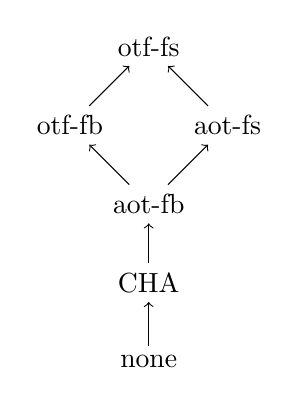
\begin{tikzpicture}
      \node (otffs) at (0, 0) {otf-fs};
      \node (otffb) at (-1, -1) {otf-fb};
      \node (aotfs) at (1, -1) {aot-fs};
      \node (aotfb) at (0, -2) {aot-fb};
      \node (cha) at (0, -3) {CHA};
      \node (none) at (0, -4) {none};

      \draw[->] (none)  -- (cha) {};
      \draw[->] (cha)   -- (aotfb) {};
      \draw[->] (aotfb) -- (otffb) {};
      \draw[->] (aotfb) -- (aotfs) {};
      \draw[->] (otffb) -- (otffs) {};
      \draw[->] (aotfs) -- (otffs) {};
    \end{tikzpicture}
  \end{center}

\caption{Relative Precision of Analysis Variations\label{FIG:LATTICE}}
\end{figure}

\begin{description}

\item[-w -app -annot-side-effect]\ \\ With these options enabled, a
simple side-effect analysis is computed using a CHA call graph and
method field read/write summaries are built. No points-to analysis is
performed to differentiate fields from different objects. Side-effect
information is then annotated in class files attributes. 

\item[-p cg.spark enabled -annot-side-effect]\ \\ 
The analysis uses Spark to compute points-to analysis. By default
it builds the call graph on-the-fly using points-to information and
performs a field-sensitive analysis. Side-effect information is then
computed using the points-to analysis, and encoded in class files.

%\item[-p cg.spark enabled,field-based -annot-side-effect]\ \\ 
%The analysis uses Spark to compute points-to analysis. By default
%it builds the call graph on-the-fly using points-to information. The
%{\tt field-based} option specifies Spark to 
%perform a field-based analysis. Side-effect information is then
%computed using the points-to analysis, and encoded in class files.

%\item[-p cg.spark enabled,on-fly-cg:false -annot-side-effect]\ \\ 
%The analysis uses Spark to compute points-to analysis. The
%{\tt on-fly-cg:false} option specifies Spark to construct the call
%graph ahead-of-time using CHA. The analysis is field-sensitive since 
%the {\tt field-based} option has a false default value. 
%Side-effect information is then
%computed using the points-to analysis, and encoded in class files.

\item[-p cg.spark enabled,on-fly-cg:false,field-based -annot-side-effect]\ \\ 
The analysis uses Spark to compute points-to analysis. The
{\tt on-fly-cg:false} and {\tt field-based} options specify Spark 
to construct the call graph ahead-of-time using CHA, and to perform a
field-based analysis.  
Side-effect information is then
computed using the points-to analysis, and encoded in class files.
\end{description}

\subsection{Examples}

Annotate class files with Soot's simple side-effect analysis. 
\begin{verbatim}
   java -Xmx400m soot.Main -w -app -annot-side-effect 
       spec.benchmarks._201_compress.Main 
\end{verbatim}

Annotate class files with a side-effect analysis using Spark. The call
graph is built ahead-of-time (aot) and the points-to analysis is field-based (fb).
\begin{verbatim}
   java -Xmx400m soot.Main -w -app -p cg.spark enabled,on-fly-cg:false,field-based 
       -annot-side-effect spec.benchmarks._201_compress.Main
\end{verbatim}

Annotate class files with a side-effect analysis using Spark. The call
graph is built ahead-of-time (aot) and the points-to analysis is
field-sensitive (fs).
\begin{verbatim}
   java -Xmx400m soot.Main -w -app -p cg.spark enabled,on-fly-cg:false 
      -annot-side-effect spec.benchmarks._201_compress.Main
\end{verbatim}

Annotate class files with a side-effect analysis using Spark. The call
graph is built on-the-fly (otf) and the analysis is
field-based (fb).
\begin{verbatim}
   java -Xmx400m soot.Main -w -app -p cg.spark enabled,field-based 
      -annot-side-effect spec.benchmarks._201_compress.Main
\end{verbatim}

Annotate class files with a side-effect analysis using Spark. The call
graph is built on-the-fly (otf) and the analysis is
field-sensitive (fs).
\begin{verbatim}
   java -Xmx400m soot.Main -w -app -p cg.spark enabled -annot-side-effect 
       spec.benchmarks._201_compress.Main
\end{verbatim}

\section{Side-Effect Attribute Format}

\begin{figure}[htbp]
\centering
\begin{minipage}{130mm}
\begin{verbatim}
SideEffectAttribute:

  RecordCount   
  (2 bytes)     
  
  BytecodeOffset   ReadSet   WriteSet   ExtraByte
  (2 bytes)        (2 bytes) (2 bytes)  (1 byte)

  BytecodeOffset   ReadSet   WriteSet   ExtraByte
  (2 bytes)        (2 bytes) (2 bytes)  (1 byte)

  ...


DependenceGraph:

  Set         Set
  (2 bytes)   (2 bytes)

  Set         Set
  (2 bytes)   (2 bytes)

  ...

\end{verbatim}
\end{minipage}
\caption{Side-Effect Attribute Format\label{FIG:SEFORMAT}}
\end{figure}

Figure~\ref{FIG:SEFORMAT} shows the format of side-effect attributes in
class files. Each method is associated with two attributes. The
first one, {\tt SideEffectAttribute}, maps each bytecode that has
side-effects to a read and write set. The extra byte contains a bit
that indicates whether a bytecode explicitly or implicitly invokes a
native method, and other bits for future use. The second attribute, 
{\tt DependenceGraph}, denotes which read and write sets have dependences. 

\section{Example of Using Side-Effect Attributes}

In Figure~\ref{FIG:SEEXAMPLE}, we show sample code and the resulting
encoding of side-effect information. Method {\tt foo} contains
instructions that, once compiled to bytecode, would include two 
{\it putfield}, two {\it invokevirtual}, and one {\it getfield} 
bytecodes at offset 2, 7, 11, 16 and 20. 
In the side-effect attribute, there is no entry for {\tt a.nothing()}
(offset 11) since this call has no side-effect. 
In method {\tt foo}, it is clear from the code that
there is a write-write dependence between statements {\tt a.g = 4} and
{\tt a.setG( 5 )}. This dependence is given in the attributes by
mapping the write set of {\tt a.g = 4} to 1 and {\tt a.setG( 5 )} to 2
in the SideEffectAttribute at offsets
7 and 16 respectively, and specifying that sets 1 and 2 have a
dependence in the DependenceGraph attribute.
Now, since there is no dependence between statements {\tt a.f = 3} and
subsequent statements, the load in statement {\tt int i = a.f} can be
eliminated by a copy of its previous assigned value (i.e. 3).

\begin{figure}[htbp]
\centering
\begin{minipage}{130mm}
\begin{Verbatim}
class A {
  int f;
  int g;
  void setF( int n ) { this.f = n; }
  void setG( int n ) { this.g = n; }
  void nothing() {}

  void foo( A a ) {
      a.f = 3;      // putfield      at offset  2
      a.g = 4;      // putfield      at offset  7
      a.nothing();  // invokevirtual at offset 11
      a.setG( 5 );  // invokevirtual at offset 16 
      int i = a.f;  // invokevirtual at offset 20
  }

  public static void main(String[] args) {
      foo( new A() );
  }
}

SideEffectAttribute (method foo): 
  RecordCount: 4
  Offset  ReadSet  WriteSet
       2       -1         0
       7       -1         1
      16       -1         2
      20        0        -1

DependenceGraph (method foo):
  Set  Set
    1    2
\end{Verbatim}
\end{minipage}
\caption{Example of Side-Effect Attribute\label{FIG:SEEXAMPLE}}
\end{figure}

          
\section*{Other information}
Our 
\htmladdnormallink{technical
report}{http://www.sable.mcgill.ca/publications/techreports/\#report2004-5}
contains detailed explanations of the side-effect variations, and how
side-effect attributes can be used in the presence of method inlining.

\section*{Change log}
\begin{itemize}
\item Feb 27, 2005: Initial version.
\end{itemize}

\end{document}

